% This template is provided for all the participants of the seminar ``Spatio-temporal Logics and Reasoning''
%%%%%%%%%%%%%%%%%%%%%
% Author information:
%%%%%%%%%%%%%%%%%%%%%
% Jannik Strötgen
% Institute of Computer Science
% Database Systems Research Group
% INF 348
% 69120 Heidelberg
% stroetgen@uni-hd.de
%%%%%%%
% Date: October 5, 2010
%%%%%%%

\documentclass[
	 11pt,         % font size
	 a4paper,      % paper format
	 oneside,
	 ]{article}

%%%%%%%%%%%%%%%%%%%%%%%%%%%%%%%%%%%%%%%%%%%%%%%%%%%%%%%%%%%%

% PACKAGES:

% Use German :
\usepackage[USenglish]{babel}
% Input encoding
\usepackage[utf8]{inputenc}
% Font encoding
\usepackage[T1]{fontenc}
% Einbinden von URLs:
\usepackage{url}
% Hyperref
\usepackage[bookmarks=true,colorlinks,pdfpagelabels,pdfstartview = FitH,bookmarksopen = true,bookmarksnumbered = true,linkcolor = black,plainpages = false,hypertexnames = false,citecolor = black,urlcolor=black]{hyperref}
%\usepackage{hyperref}
% Include Graphic-files:
\usepackage{graphicx}
% Include PDF links
%\usepackage[pdftex, bookmarks=true]{hyperref}
% Fuer Textsatz
\usepackage{setspace}
% For bibliography style
\usepackage[numbers]{natbib}
% for Latex symbols
\usepackage{ marvosym }
% tables
\usepackage{ tabularx }
% quates
\usepackage[babel,german=quotes]{csquotes}
% colors
\usepackage[usenames, dvipsnames]{xcolor}
% subscript
% \usepackage{fixltx2e}
% verzeichnisse zu toc hinzufügen
\usepackage{tocbibind}
% index
\usepackage{makeidx}
\usepackage{showidx} %DEBUG: remove
% placement H for exactly here!
\usepackage{float}
% strikeout text
\usepackage[normalem]{ulem}
% tightly packed lists
\usepackage{mdwlist}
% long tables
\usepackage{longtable}
% better ruler support for tables
\usepackage{booktabs}
% source code highliting
\usepackage{minted}
% background color for listings
\definecolor{bg}{rgb}{0.95,0.95,0.95}
% neat quotes everywhere
\usepackage{epigraph}
\setlength\epigraphwidth{12cm}
\setlength\epigraphrule{0pt}
% for a glossary
\usepackage[toc]{glossaries}
\makeglossaries

\newglossaryentry{X3D}{
  name=X3D,
  description={An XML based scene description language and the successor of \gls{VRML}}
}
\newglossaryentry{Roundtrip3D}{
  name=Roundtrip3D,
  description={Aim to extend SSIML, a MDD approach for 3D development to full round-trip engineering. \cite{roundtrip3dwebsite}}
}

\newacronym{GPU}{GPU}{Graphical Processing Unit}
\newacronym{SVG}{SVG}{Scalable Vector Graphics}
\newacronym{R3D}{R3D}{Roundtrip3D}
\newacronym{SSIML}{SSIML}{Scene Structure and Integration Modelling Language}

\newglossaryentry{SceGraToo}{
  name=SceGraToo,
  description={\textbf{Sce}ne \textbf{Gra}ph Composition \textbf{Too}l}
}
\newglossaryentry{OpenGL}{
  name=OpenGL,
  description={Open Graphics Library. An environment for developing portable, interactive 2D and 3D graphics applications. \cite{opengl}}
}
\newglossaryentry{git}{
  name=git,
  description={A free and open source distributed version control system designed to handle everything from small to very large projects with speed and efficiency. \cite{git}}
}
\newglossaryentry{WebGL}{
  name=WebGL,
  description={A cross-platform, royalty-free web standard for a low-level 3D graphics API based on OpenGL ES 2.0. \cite{webgl}}
}
\newacronym{3D}{3D}{3 Dimensial}
\newacronym{DAG}{DAG}{Directed Acyclic Graph}
\newacronym{XML}{XML}{Extensible Markup Language}
\newacronym{VRML}{VRML}{Virtual Reality Modeling Language}
\newacronym{HTML}{HTML}{Hypertext Transfer Protocol}
\newacronym{JSON}{JSON}{JavaScript Object Notation}
\newacronym{ID}{ID}{Identifier}
\newacronym{DOM}{DOM}{Document Object Model}

% caption* for unnumbered captions
\usepackage{caption}

%%%%%%%%%%%%%%%%%%%%%%%%%%%%%%%%%%%%%%%%%%%
% Titel, Autor, Seminar, Semester, Dozent %
%%%%%%%%%%%%%%%%%%%%%%%%%%%%%%%%%%%%%%%%%%%
\newcommand{\mytitle}{Web-based 3D-scene composition for further server-sided processing in the Roundtrip3D project}
\newcommand{\mytitleShort}{SceGraToo}
\newcommand{\myauthor}{Danny Arnold}
\newcommand{\myseminar}{Web-basierte Komposition von 3D-Szenen für deren serverseitige Weiterverarbeitung im Roundtrip3D Projekt}
\newcommand{\mydozent}{Prof. Jung}
\newcommand{\mydozentTwo}{Matthias Lenk}
\newcommand{\myseminarTwo}{serverseitige Weiterverarbeitung im Roundtrip3D Projekt}
\newcommand{\mysemester}{Summer Semester 2015}

% OTHER SETTINGS:
% \setlength{\parindent}{0in}
\renewcommand{\arraystretch}{1.5}

% add listoflistings to the toc
\renewcommand{\listoflistings}{
  \cleardoublepage
  \addcontentsline{toc}{section}{\listoflistingscaption}
  \listof{listing}{\listoflistingscaption}
}

\newcommand{\emptypage}[0]{
	% Empty Page
	\clearpage
	\thispagestyle{empty}
	\mbox{}
	\newpage
}

\newcommand{\headingspage}[0]{
	% Empty Page
	\clearpage
	\thispagestyle{headings}
	\mbox{}
	\newpage
}

% Pagestyle:
\pagestyle{myheadings}
\markright{\myauthor: \mytitleShort}

% start indexing
\makeindex

\begin{document}

%%%%%%%%%%%%%%%%%%%%%%%%%%%%%%%%%%%%% <TITLE> %%%%%%%%%%%%%%%%%%%%%%%%%%%%%%%%%%%%%
\pagenumbering{roman}
\begin{titlepage}
\begin{tabular}[l]{l}
% Angaben zum Seminar
TU Bergakademie Freiberg\\
Faculty for Mathematics and Computer Science\\
\mysemester\\
German Title: \myseminar\\
\phantom{German Title: }\myseminarTwo\\
Supervisor: \mydozent\\
\phantom{Supervisor: }\mydozentTwo\\
\end{tabular}

\vspace{4cm}
\begin{center}
\textbf{\large Bachelor Thesis} % Proseminararbeit,Studienarbeit, Interdisziplinaeres Projekt
\vspace{0.5\baselineskip}

% Titel wird ausgegeben (siehe oben)
{\huge
\mytitle
}
\end{center}

\vfill
% Persönliche Angaben
\begin{tabular}[l]{ll}
Name:           & \myauthor\\
Matriculation Number: & 52315\\
Major:    & Applied Computer Science\\
Email: & danny.arnold@student.tu-freiberg.de\\
Date: & \today \\
\end{tabular}

\end{titlepage}
\newpage
%%%%%%%%%%%%%%%%%%%%%%%%%%%%%%%%%%%%% </TITLE> %%%%%%%%%%%%%%%%%%%%%%%%%%%%%%%%%%%%

\emptypage

% Zeilenabstand
\onehalfspacing


%%%%%%%%%%%%%%%%%%%%%%%%%%%%% <Antiplagiatserklärung> %%%%%%%%%%%%%%%%%%%%%%%%%%%%%
\thispagestyle{empty}
\vspace*{100pt}
I, \textbf{\myauthor}, declare that I have read and understood
the material exemplifying and explaining cases of plagiarism, and that my paper contains no plagiarized
material and is solely my own work. I am aware of the fact that should my paper be found to
contain plagiarized material or to have been written in part or whole by someone else, this will
entail serious consequences. These include the following:
1. The reason for my failure will be recorded by the department.
2. I will not be given credit for the course.
3. The Honor Board may review my paper and suggest additional sanctions, including
expulsion.
Furthermore, I am aware that submitting the same or a revised paper in two separate courses without
the instructors' explicit consent will result in similar consequences.\cite{Antiplagiatserklrung}
\vspace*{50pt}

Freiberg, \today \hspace{2cm} \underline{\phantom{Platz für die Unterschrift}}
\clearpage
%%%%%%%%%%%%%%%%%%%%%%%%%%%%% </Antiplagiatserklärung> %%%%%%%%%%%%%%%%%%%%%%%%%%%%%

%%%%%%%%%%%%%%%%%%%%%%%%%%%%%% <Danksagung> %%%%%%%%%%%%%%%%%%%%%%%%%%%%%%%%%%%%%%%%
% TODO: translate
\emptypage
\thispagestyle{empty}
\section*{Acknowledgment} % (fold)
\label{sec:danksagung}

% Danken möchte ich allen voran \mydozent \index{Froitzheim} und \mydozentTwo \index{Jasper} für dieses Seminar und all ihre Hilfe. Des Weiteren möchte ich mich bei \citeauthor{SeminarTemplate} für sein sehr gutes Latex-Template \cite{SeminarTemplate} bedanken, welches dieser Arbeit zu Grunde liegt, aber in vielen Bereichen angepasst wurde. Eine weitere sehr große Hilfe war das WikiBook \LaTeX~\cite{WikiLatex}, auch vielen Dank an alle Autoren dieses WikiBooks. \\

% Mein Dank geht auch an die fleißigen Korrekturleser Friederike Klos \index{Klos, Friederike} und Felix Kästner \index{Kästner, Felix}.

% Thanks!

\begin{figure}[htbp]
	
\includegraphics[width=\textwidth]{../assets/my-little-pony-mlp-other-261396.jpeg}
\end{figure}

% section danksagung (end)

%%%%%%%%%%%%%%%%%%%%%%%%%%%%%% <Inhaltsverzeichnis> %%%%%%%%%%%%%%%%%%%%%%%%%%%%%%%%
\emptypage
% Table of contents
\setcounter{tocdepth}{5}
\tableofcontents
\clearpage
%%%%%%%%%%%%%%%%%%%%%%%%%%%%%% </Inhaltsverzeichnis> %%%%%%%%%%%%%%%%%%%%%%%%%%%%%%%

%%%%%%%%%%%%%%%%%%%%%%%%%%%%%% <Hauptteil der Arbeit> %%%%%%%%%%%%%%%%%%%%%%%%%%%%%%
\emptypage
\pagenumbering{arabic}

% !TEX root = seminararbeit.tex

\section{Introduction}
\label{sec:Prelude}

The goal of the thesis is to create an editor for \acr{3D} scenes, using web technologies,
which enables its users to post-process \gls{X3D} scenes. These scenes are the
product of a tool that was implemented as part of the DFG research
project \gls{R3D} \cite{Jung:2015:SDA:2802768.2802837}.
% The scene are automatically derived from software models \ldots{}
\subsection{Motivation}\label{motivation}

As part of the \gls{R3D} project, a round-trip framework
was developed. This framework also includes a
graphical editor for \acr{SSIML} \cite{Lenk:2012:MID:2338714.2338742} models, to describe \gls{3D} applications. Then
\gls{R3D} can be used to generate boilerplate code for multiple programming
languages, such as JavaScript, Java or C++, and an \gls{X3D} file describing
the scene. The \gls{X3D} file may contain references to other \gls{X3D} files
containing the actual \gls{3D} data (e.g.~a car and its corresponding tires),
hereafter called \emph{inlines}. These files are created by exporting
objects from a \gls{3D} computer graphics software (e.g.~Blender,
Maya or 3DS Max).\\
The problem that arises is that each object is usually in the center of
its own coordinate system. So they need to be translated, rotated and
maybe even scaled, to result in the desired scene (e.g.~a car where the tires
are in the places they belong to and not in the center of the chassis).
The scene structure (see Listing \ref{list:x3dscene}) is mostly generated. Attribute values of respective nodes,
such as transform nodes, need to be adjusted in order to compose the
overall \gls{3D} scene.

% \includegraphics{Figure of a car with the tires in the center}\\
% \includegraphics{Figure of a car with the tires where they belong to}

This can be achieved by adjusting \emph{translate}, \emph{rotate} and
\emph{scale} properties to arrange \gls{3D} objects. To exacerbate this problem
further, the orientation the \gls{3D} artists chose for its object may be unknown if
there is no convention for \gls{3D} modeling. The main problem is, that \gls{3D} transformations, such as translation,
orientation and scale of single \gls{3D} geometries, need to be adjusted. So far,
there is no graphical tool that meets both of the following requirements:

\begin{itemize*}
  \item User friendly and straight forward composition functionalities for \gls{X3D} scenes and
  \item preservation of (generated) information, such as node names or comments (necessary to merge the changed files back into the source model).
\end{itemize*}

\begin{figure}
  \begin{minipage}{.5\textwidth}
    \centering
    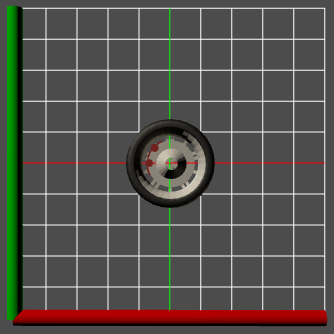
\includegraphics[width=0.9\textwidth]{../assets/wheel1.png}\\
    a)
  \end{minipage}
  \begin{minipage}{.5\textwidth}
    \centering
  	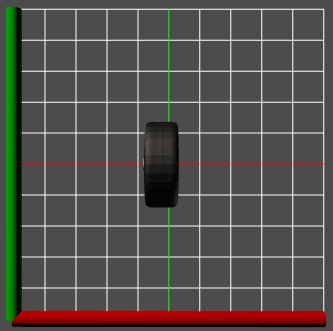
\includegraphics[width=0.9\textwidth]{../assets/wheel2.png}\\
    b)
  \end{minipage}\\
  \begin{minipage}{.5\textwidth}
    \centering
  	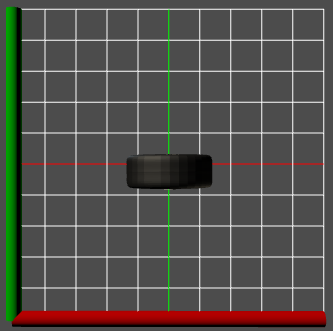
\includegraphics[width=0.9\textwidth]{../assets/wheel3.png}\\
    c)
  \end{minipage}
  \begin{minipage}{.5\textwidth}
    \centering
  	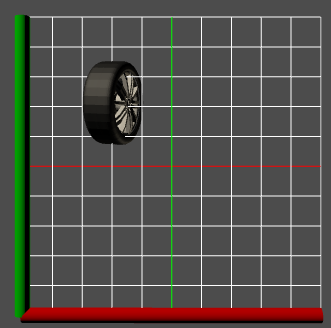
\includegraphics[width=0.9\textwidth]{../assets/wheel4.png}\\
    d)
  \end{minipage}
  \caption{Figures \ref{fig:wheel}a-c show common orientations the \gls{3D} model of a wheel could have. Figure \ref{fig:wheel}d shoes the worst case.}
	\label{fig:wheel}
\end{figure}

Figure \ref{fig:wheel} demonstrates multiple orientations a \gls{3D} model of a wheel can have. Figures \ref{fig:wheel}a-c are common
orientations, since it is disputable which of these could be considered the
norm. But if one depends on art from 3rd parties, the orientation and position
could be completely arbitrary like in Figure \ref{fig:wheel}d).

These properties could be added and adjusted via any text editor by opening the
generated \gls{X3D} file, but the resulting work-flow is not user-friendly. The
following list explains the work-flow using just a text editor.

\begin{enumerate*}
  \item Model the \gls{3D} application, including the \gls{3D} scene structure.
  \item Generate the \gls{3D} scene and the application code.
  \item Run the application and evaluate the scene and think about what objects need to go where and whether they need to be scaled.
  \item Type random translation, rotation and scale values into the transform nodes.
  \item Run the application again and evaluate whether the transformations are correct (since one does not know anything about the orientation of the object).
  \item Go back to 4. until all objects are placed correctly.
\end{enumerate*}

Tools like Maya or Blender could be used for this, but their import
and export filters discard important meta-data that is necessary for the
round-trip transformation. This is what \gls{SceGraToo} is meant to be. \gls{SceGraToo} addresses both of these issues. It allows for loading the root \gls{X3D} file and changing all transformations, containing the inline nodes,
using mouse interactions. For fine grained control \gls{SceGraToo} also
contains a tree view that allows the user to input exact attributes for
translations, rotations and scale (see Figure \ref{fig:tree-view}).

\subsection{Scope}\label{scope}

The provided application (\gls{SceGraToo}) addresses two issues:

\begin{enumerate*}
  \item Allowing the composition of generated \gls{X3D} scenes (with focus on usability). E.g., accompanying the \gls{3D} view, a tree view for fine grained editing, that should not only visualize the \gls{3D} scene's structure, but also allow for entering concrete coordinate values.
  \item During the editing process, the preservation of all information/meta-data must be guaranteed.
\end{enumerate*}


% !TEX root = seminararbeit.tex

\section{Basics and Related Work}
\label{basics-and-related-work}

\subsection{Scene-Graph}\label{scene-graph}

Scene-graphs can be used to group and organize \gls{3D} objects, their properties and
concerning transformations. A gls{DAG} can be used to represent a scene-graph.
It starts with a root node that is associated with one or more children. Each
child can be an object or a group, again containing more children. A group can
contain associated transformation information, like \emph{translation},
\emph{rotation} or \emph{scaling}. This structure has certain advantages
compared to applying all transformations to the raw meshes and sending
everything to the \gls{GPU}. \cite{realityprime} \gls{SSIML} \cite{Lenk:2012:MID:2338714.2338742} scene-graphs differ from the
above definition and there are three types of nodes:

\begin{itemize*}
  \item Transform nodes,
  \item geometry nodes and
  \item group nodes.
\end{itemize*}

\subsubsection{Culling}\label{culling}

Before using structures like scene-graphs, all polygons would be sent to
the \gls{GPU} and the \gls{GPU} would need to test which polygons are actually in the
view and thus need to be rendered. The problem of this approach is
that this information was only known after doing a lot of calculations
for every polygon already.\\
With a scene-graph it is possible to start from the root and traverse the
graph, testing the bounding box of each group and only sending it to the
\gls{GPU} if it is completely visible. If it is not, the whole sub-tree is not
sent to the \gls{GPU}. If it is partially visible the same process is applied
to the sub-tree.\\
By using a structure that retains more information about what it
represents it is possible to let the CPU do more of the heavy
lifting and unburden the \gls{GPU}.

\begin{quote}
  Rather than do the heavy work at the \gls{OpenGL} and polygon level,
  scene-graph architects realized they could better perform culling at
  higher level abstractions for greater efficiency. If we can remove the
  invisible objects first, then we make the hardware do less work and
  generally improve performance and the all-important frame-rate. \cite{realityprime}
\end{quote}

\subsubsection{Transformations}\label{transformations}

Another advantage is the way transformations work. Instead of applying
them to the meshes directly, and keeping track of what meshes belong to
the same object (like the chassis, the tires and the windows of a
car), they can simply be nested under the same transformation group. The
transformation thus applies to all objects associated with that group.

\subsubsection{Reuse}\label{reuse}

With the ability to address nodes it is possible to reuse their
information. If you have a car, it would be enough to have only one node
containing the geometry for a tire, all other tires are merely addressing
the tire with the geometry information (see listing \ref{list:defuse}).
That way the memory footprint of an application can be reduced.

\begin{listing}
  \begin{minted}[breaklines,bgcolor=bg]{html}
<Group>
  <Transform>
    <Shape def="chassis">
        <Appearance>
            <Material></Material>
        </Appearance>
        <Box></Box>
    </Shape>
  </Transform>
  <Transform>
    <Shape def="tire">
        <Appearance>
             <Material></Material>
        </Appearance>
        <Torus></Torus>
    </Shape>
  </Transform>
  <Transform>
    <Shape use="tire"/>
  </Transform>
  <Transform>
    <Shape use="tire"/>
  </Transform>
  <Transform>
    <Shape use="tire"/>
  </Transform>
</Group>
  \end{minted}
  \caption{Example \gls{X3D} group showing the use of \texttt{def} and \texttt{use}.}
  \label{list:defuse}
\end{listing}


\subsection{X3D}
\label{x3d} \gls{X3D} \cite{x3d} is the \gls{XML} representation of \gls{VRML} which was designed as a
universal interactive \gls{3D} exchange format, much like \gls{HTML} is for written
documents or \gls{SVG} for vector graphics. Due to its \gls{XML} structure it can be
integrated in \gls{HTML} documents, thus the Frauenhofer Institute pursued to
implement a runtime that could interpret and visualize \gls{X3D} in the browser, by
using a \gls{WebGL} context. It is called x3dom \cite{x3dom} and it is extensively used
by SceGraToo, the tool that arose from this thesis.

\subsection{x3dom}
\label{par:x3dom}

As said in the previous section, x3dom was developed by the Frauenhofer
Institute to realize the vision that started \gls{VRML} in the first place: \emph{mark
up interactive \gls{3D} content for the web}. On the web there are two entirely
different approaches to describe the same thing:

\begin{itemize*}
  \item imperative
  \item declarative
\end{itemize*}

\begin{longtable}[c]{@{}lll@{}}
  \caption{The matrix in this table classifies x3dom together with other common web technologies \cite{x3dom}.\label{tab:feature_matrix}}\\
  \toprule
  & 2D & \gls{3D} \tabularnewline
  \midrule
  \endhead
  Declarative & \gls{SVG} \cite{svg} & x3dom \cite{x3dom} \tabularnewline
  Imperative  & Canvas \cite{canvas} & \gls{WebGL} \cite{webgl} \tabularnewline
  \bottomrule
\end{longtable}

As can be seen in table \ref{tab:feature_matrix} x3dom complements the already existing technologies
perfectly.

\clearpage
\subsection{SSIML}
\label{ssiml}

Heterogeneous developer groups, groups that are comprised of people from
different backgrounds (programmers, \gls{3D} designers) have their difficulties
working together. They work in different domains and use different tools
adjusted to that domain. \cite{Glinz:2015:SUS:2802768.2802838}

SSIML is a graphical approach to unify the scene-graph model and the the
application model, thus making the communication between the different
parties easier.

It also serves as a code generation template.

\begin{figure}
  \centering
  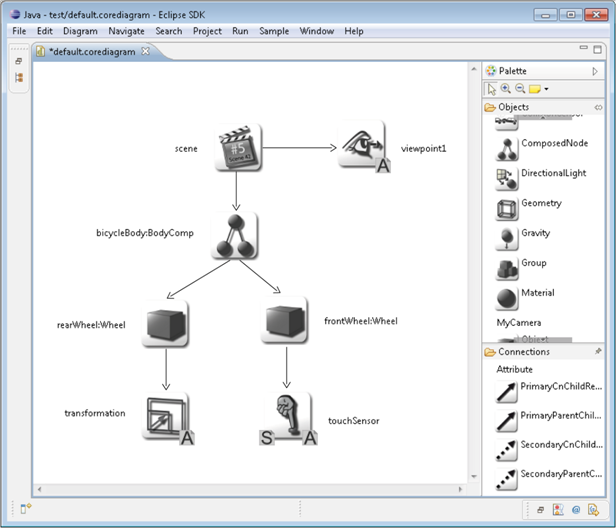
\includegraphics[width=12cm]{../assets/SSIML.png}
	\caption{This figure shows the graphical editor for SSIML. In particular it shows a scene comprising a bike. \cite{roundtrip3dwebsite}}
	\label{fig:ssimldiagram}
\end{figure}

\subsection{Roundtrip 3D}\label{roundtrip-3d}

As stated above, when developing \gls{3D} applications, many different
developers are involved, i.e.~\gls{3D} designers, programmers and, ideally,
also software designers (see figure \ref{fig:ssimldiagram}).

% TODO: convert to pdf
% 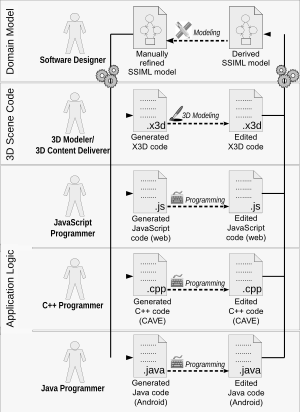
\includegraphics{../assets/csrd2014.svg}\\
% Roundtrip3D proposed process
% \href{http://dx.doi.org/10.1007/s00450-014-0258-8}{JLV15}

Roundtrip3D was a research project that, amongst others, resulted in a
graphical editor for \hyperref[ssiml]{SSIML} models. It offers an
approach for merging a developer's changes back into the main model.
After all working copies are merged back into the main model (dropping
unwanted or conflicting changes), all working copies are regenerated and
delivered to the individual developers. After each roundtrip every
developer has a copy of the project that is consistent with everyone
else's.

\subsection{Related Work}
\label{related-work}

The next section examines efforts and applications in the field of

\begin{itemize*}
  \item collaborative remote working on \gls{3D} models and
  \item online \gls{3D} editors.
\end{itemize*}

\subsubsection{3D Meteor}
\label{d-meteor0}

\begin{figure}[htbp]
  \centering
  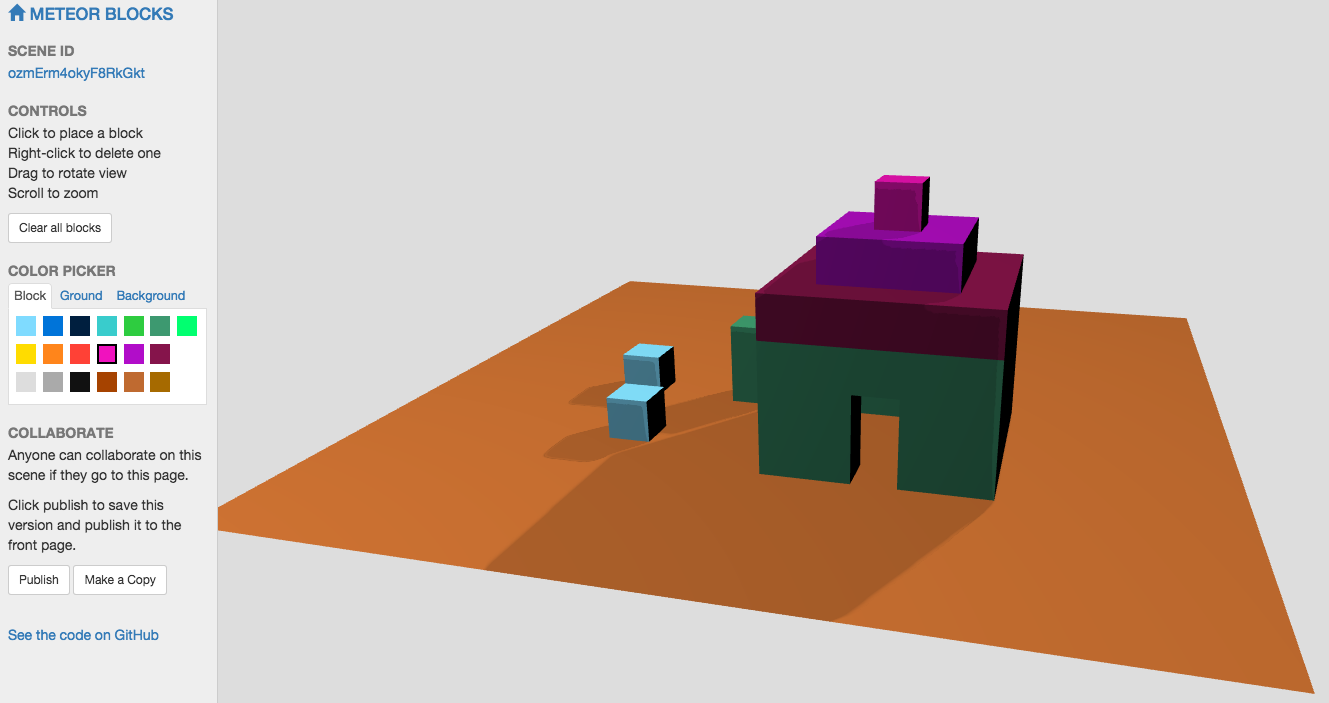
\includegraphics[width=12cm]{../assets/3dmeteor.png}
  \caption{This is a scene in 3dmeteor showing a house and a garden of cubes.}
	\label{fig:3dmeteor}
\end{figure}

This simple \gls{3D} editor allows the user to add and remove colored blocks to a
scene. The synchronization is leveraging meteor's database collection
subscription features. Meteor applications are comprised of a client side and a
server side. The client can subscribe to database collections and gets
automatically notified of changes to that collection by the server. The only
thing that actually is synchronized is an array of \emph{boxes}. A box is an
object with an x, y and z property describing its position. When a box is
added to the collection the collection is synchronized with the server. The
server informs all other browser instances that show this scene of the new box.
These browser instances reevalute the template that renders the x3dom scene to
the \gls{DOM} and the the \gls{DOM} is updated to contain the new box, thus synchronizing
the scene with the browser instance. \cite{3dmeteor}

\subsubsection{Blender Plugin}
\label{blender-plugin}

As part of an asset management system the Université du Québec à
Montréal implemented a plugin for Blender for collaborative working. An
artist can record changes to wiremeshes and store them on a server.
Another artist can download these changes and apply them to his working
copy. The change sets are a simple list of vertices and their movement in the
x, y and z space (see listing \ref{blenderplugin}). \cite{LCR07}

\begin{listing}
  \begin{minted}[breaklines,bgcolor=bg]{text}
95 [0.0000, 0.0000, 0.0000]
295 [0.0027, 0.0013, 0.0000]
309 [0.2123, 0.1001, 0.0000]
311 [0.3029, 0.1429, 0.0000]
  \end{minted}
  \caption{This shows a change set of 4 polygons and how they where moved.}
  \label{blenderplugin}
\end{listing}

These are saved on the server and another user working on the same
object can apply them to his working copy. They can actually be applied
to any object that has the same number of vertices. That is also a
shortcoming. Adding or removing vertices cannot be handled by the
plugin. It is also not in real time, so it is more comparable to version
control system like \gls{git} just for \gls{3D} models.

\subsubsection{Gizmos}\label{gizmos}

Gizmos, also called manipulators, are handles or bounding boxes with
handles that manipulate their containing objects in a predefined way when
dragged. \cite{wikigizmo}

In \gls{X3D} gizmos can be realized with specialized X3DDragSensorNodes \cite{x3ddragsensornode}, like:

\begin{description*}
\item[SphereSensor]
  SphereSensor converts pointing device motion into a spherical rotation around the origin of the local coordinate system. \cite{spheresensor}
\item[CylinderSensor]
  The CylinderSensor node converts pointer motion (for example, from a mouse) into rotation values, using an invisible cylinder of infinite height, aligned with local Y-axis. \cite{cylindersensor}
\item[PlaneSensor]
  PlaneSensor converts pointing device motion into 2D translation, parallel to the local Z=0 plane. Hint: You can constrain translation output to one axis by setting the respective minPosition and maxPosition members to equal values for that axis. \cite{planesensor}
\end{description*}

The sensors track drag events on their siblings. In the example in figure
\ref{fig:x3dgizmo} (which is taken directly from the x3dom website) the
PlaneSensor tracks drag events on the cones and the cylinder that make up the
cyan handle. Part of the structure of the scene can be seen in listing
\ref{planesensor}.

Every time it detects a drag event it converts it into a 2D
transformation and raises an \texttt{onOutPutChange} event.\\
The callback \texttt{processTranslationGizmoEvent} is registered as an event handler.
In this function the position of the handle is adjusted to make it
follow the drag movement, also the position of the teapot is adjusted.

Having the handles being \gls{3D} objects within the scene, that look
touchable and intractable, make it easier for users find their way
around the application. Instead of having to learn keyboard shortcuts
users simply use their intuition and knowledge about how to interact with
objects in the real world.

The pictures in \ref{blender} to \ref{fig:x3dgizmo} show different gizmos from
different applications.

\begin{listing}
  \begin{minted}[breaklines,bgcolor=bg]{html}
<group>
  <planeSensor autoOffset='true' axisRotation='1 0 0 -1.57' minPosition='-6 0' maxPosition='6 0' onoutputchange='processTranslationGizmoEvent(event)'>
  </planeSensor>

  <transform id='translationHandleTransform'>
    <transform translation='0 -5.5 8' rotation='0 1 0 1.57'>
      <transform translation='0 0 1.5' rotation='1 0 0 1.57'>
        <shape DEF='CONE_CAP'>
          <appearance DEF='CYAN_MAT'><material diffuseColor='0 1 1'></material></appearance>
          <cone height='1'></cone>
        </shape>
      </transform>
      <transform rotation='1 0 0 -1.57'>
        <shape>
          <appearance USE='CYAN_MAT'></appearance>
          <cylinder></cylinder>
        </shape>
      </transform>
      <transform translation='0 0 -1.5' rotation='1 0 0 -1.57'>
        <shape USE='CONE_CAP'></shape>
      </transform>
    </transform>
  </transform>
</group>
  \end{minted}
  \caption{This shows a group containing a planeSensor. It shows a part of the scene depicted in figure \ref{fig:x3dgizmo}.}
  \label{planesensor}
\end{listing}

\begin{figure}[htbp]
  \begin{minipage}{.5\textwidth}
    \centering
    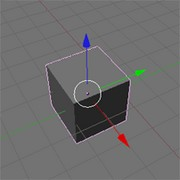
\includegraphics[width=0.9\textwidth]{../assets/Manual-Manipulators-Translate.jpg}\\
  	a) A translation gizmo. \cite{blenderwiki}
  \end{minipage}
  \begin{minipage}{.5\textwidth}
    \centering
    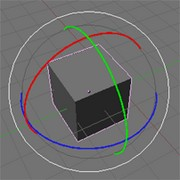
\includegraphics[width=0.9\textwidth]{../assets/Manual-Manipulators-Rotate.jpg}\\
  	b) Rotation gizmo. \cite{blenderwiki}
  \end{minipage}\\
  \begin{minipage}{.5\textwidth}
    \centering
    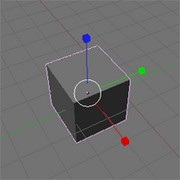
\includegraphics[width=0.9\textwidth]{../assets/Manual-Manipulators-Scale.jpg}\\
  	c) Scale gizmo. \cite{blenderwiki}
  \end{minipage}
  \begin{minipage}{.5\textwidth}
    \centering
    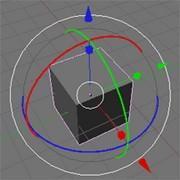
\includegraphics[width=0.9\textwidth]{../assets/Manual-Manipulators-Combo.jpg}\\
  	d) All gizmos together. \cite{blenderwiki}
  \end{minipage}
  \caption{The same cube in Blender with different gizmos/transformers enabled.}
  \label{blender}
\end{figure}
\begin{figure}[]
  \centering
  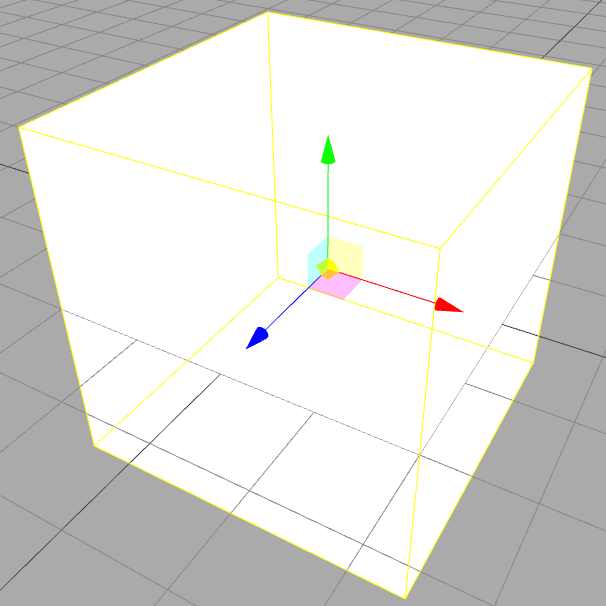
\includegraphics[width=12cm]{../assets/threejs-editor.png}
	\caption{ Shows translate gizmos along the x, y and z axis as well as gizmos that translate the cube along the xy, xz, yz and frustum plane. \cite{threejseditor} }
\end{figure}
\begin{figure}[]
  \centering
  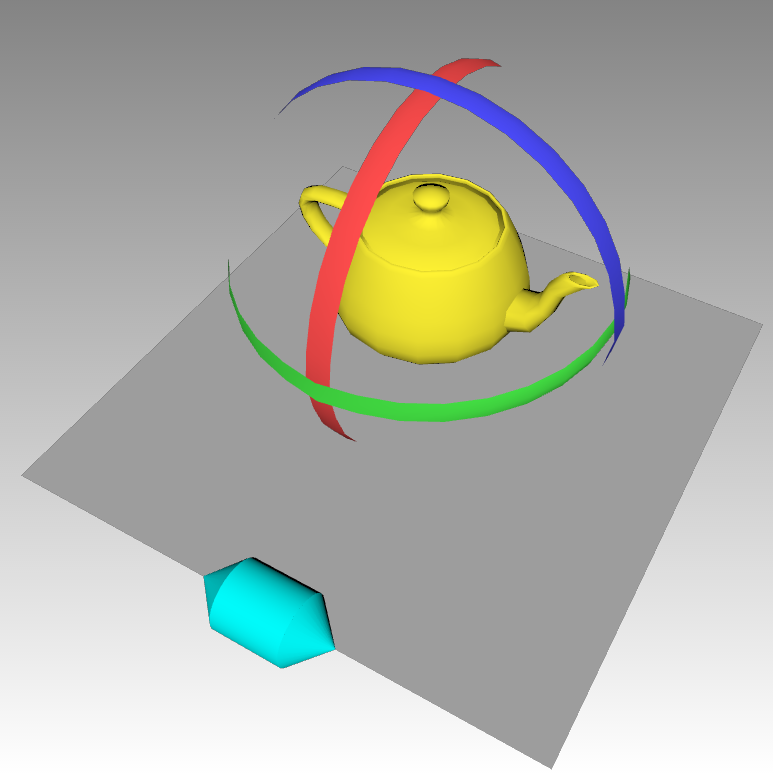
\includegraphics[width=12cm]{../assets/x3dom-gizmo-example.png}
	\caption{ Shows an official x3dom tutorial for using sensors to create gizmos. \cite{x3dgizmo} }
	\label{fig:x3dgizmo}
\end{figure}

\clearpage

\subsubsection{Component Editor}
\label{component-editor30}

On the 12th of June 2015 the x3dom maintainers released their Component Editor. \cite{componenteditor}
It was released after the the work on \gls{Roundtrip3D} started.
Its development took about a year and three people working part-time on it. \cite{componenteditoreffort}
Although it does offer all the wanted scene composition features, it lacks the ability to:

\begin{itemize*}
  \item Load an existing \gls{X3D} file,
  \item save the scene as an \gls{X3D} file and
  \item upload \gls{X3D} files that can be included as inlines.
\end{itemize*}

Scenes can only be loaded and saved as a \gls{JSON} representation (see listing~\ref{componenteditorjson}).
Conversion between the formats may be possible, but meta information like \gls{ID}s in comments would be lost.

\begin{listing}
  \begin{minted}[breaklines,bgcolor=bg]{json}
{
  "0": {
    "type": "Box",
    "transform": "1.000000, 0.000000, 0.000000, 0.000000, \n0.000000, 1.000000, 0.000000, 0.000000, \n0.000000, 0.000000, 1.000000, 0.000000, \n0.000000, 0.000000, 0.000000, 1.000000",
    "referencePoints": ["p1", "p2", "p3", "p4", "p5", "p6"],
    "parameters": {
      "Size": [1, 1, 1],
      "Positive Element": "true"
    }
  }
}
  \end{minted}
  \caption{The \gls{JSON} format used by the component editor to save scenes.}
  \label{componenteditorjson}
\end{listing}

\subsubsection{Real-Time Collaborative Scientific WebGL Visualization with Web Sockets}
\label{rtcswvwws}

Using web sockets instead of AJAX is an interesting approach.
\cite{Marion:2012:RCS:2338714.2338721} Especially the cut down on latency. It is
over all very similar to the approach that was considered for SceGraToo, but not
implemented due to time constraints. In the end the differences between
SceGraToo's requirements and theirs outweigh the similarities. \gls{Roundtrip3D} not only
has to visualize a scene, but also manipulate it. And to achieve a spector mode
like in this work not only the viewpoint would have to be synchronized but also
the whole scene. This can either be done by sending the whole scene to the other
clients on every change, or sending change sets, which poses an interesting
challenge. They visualize a specific dataset in a threejs's specific \gls{JSON} format
\cite{threejs-format}. \gls{Roundtrip3D} only needs to render \gls{X3D} scenes, converting the
scene into another format and have it rendered by another scene graph framework
is unnesesary, since x3dom does a pretty good job doing this.

\subsubsection{ParaViewWeb}
\label{paraviewweb-pvweb}

Simple to use out of the box, but needs a paraview server instance and
paraview does not support \gls{X3D} as an input format. So using this is unfortunately
not possible unless an import filter is written. The visualization is
mainly meant to explore data sets. There is no easy way to manipulate
the input data. This can only happen by extending the visualization
pipeline via python scripts on the server.


% !TEX root = seminararbeit.tex

\section{Concept}
\label{concept}

% TODO: skizze wie dom rendering funktioniert oder auch nicht, da es ziemlich uninteressant ist

In the following sections the initial design concept of \gls{SceGraToo} is illustrated.

\subsection{Server}
\label{server}

\subsubsection{Node.js}
\begin{quote}
  ``Node.js is a platform built on Chrome's JavaScript runtime for easily building fast, scalable network applications. Node.js uses an event-driven, non-blocking I/O model that makes it lightweight and efficient, perfect for data-intensive real-time applications that run across distributed devices.'' \cite{nodejs}
\end{quote}

Node is used because it is inherently easy writing small servers with it, and
SceGraToo's server is not going to be complex. \footnote{Complex servers can be
written in Node.js as well, it is just not encouraged, since most people tend to
refactor their infrastructure into micro services.}

Listing \ref{list:nodejs} shows a server that is looking up a user from the database and returning it as \gls{JSON} to the browser.

\begin{listing}
  \begin{minted}[breaklines,bgcolor=bg]{javascript}
const http = require('http')
const db = require('db')

http.createServer((request, response) => {
  db.getuser(function(error, user) {
    if (error) {
      return res.status(404).send(error);
    } else {
      response.writeHead(200, {'Content-Type': 'application/json'})
      response.send(user)
    }
  })
}).listen(1337, '127.0.0.1')
  \end{minted}
  \caption{an example server in Node.js, using the http module in its standard library}
  \label{list:nodejs}
\end{listing}

\subsubsection{Koa}
\label{par:Koa}
\begin{quote}
  ``Koa is a new web framework designed by the team behind Express, which aims to be a smaller, more expressive, and more robust foundation for web applications and APIs. Through leveraging generators Koa allows you to ditch callbacks and greatly increase error-handling. Koa does not bundle any middleware within core, and provides an elegant suite of methods that make writing servers fast and enjoyable.'' \cite{koajs}
\end{quote}

Koa is used to make writing the server and using asynchronouse functions in request handlers even simpler and clearer.
See listing \ref{list:koajs} for the same example from listing \ref{list:nodejs} written with koajs.
It is not only shorter, but also simplier and clearer.

\begin{listing}
  \begin{minted}[breaklines,bgcolor=bg]{javascript}
const db = require('db')
const koa = require('koa')
const app = koa()

app.use(function * (){
  this.body = yield db.getUser()
})

app.listen(3000)
  \end{minted}
  \caption{an example server utilizing the koajs framework}
  \label{list:koajs}
\end{listing}

\subsection{Client}
\label{client}

\epigraph{I conclude that there are two ways of constructing a software design:
One way is to make it so simple that there are obviously no deficiencies
and the other way is to make it so complicated that there are no obvious
deficiencies. The first method is far more difficult.}{--- Hoare, Turing Award Lecture 1980}

The tree-view is the most important part of SceGraToo, it shows the
the structure rather than the visual representation. Different
off-the-shelf solutions, like angular or JQuery plugins, were tested
against the following requirements:

\begin{enumerate*}
  \item Custom \gls{HTML} elements as part of tree nodes (e.g.~multiple checkboxes or multiple inputs),
  \item ability to observe the tree node's state changing,
  \item binding to an arbitrary model and
  \item detecting inconsistencies between the model and the view and recovering from them.
\end{enumerate*}

\textbf{Partially not met requirements:}

\begin{itemize*}
  \item Custom elements as part of tree nodes and
  \item ability to listen to changes to the tree node.
\end{itemize*}

\textbf{Requirements none of the tested tools met:}

\begin{itemize*}
  \item Binding to an arbitrary model and
  \item detecting inconsistencies between the model and the view and recovering from them.
\end{itemize*}

None of the off-the-shelf solutions could satisfy all expectations. After
evaluating a couple of solutions it was clear that the problem space was too
specific and a custom solution is required.

\subsubsection{Synchronization Process}

Of all requirements, the most complicated part is keeping the tree-view in sync
with the scene-graph while the scene-graph is being modified and vice
versa.

\paragraph{Terminology}
\label{terminology}

\begin{description*}
  \item[scene-graph]
    The \gls{X3D} representation of the scene as part of the \gls{DOM}, see listing~\ref{list:x3dscene} and the screenshot in figure \ref{fig:x3dom-dom} from the Chrome DevTools.
  \item[scene-graph-node]
    A specific scene graph node (e.g.~\texttt{inline}, \texttt{transform} or \texttt{scene}).
  \item[tree-view-component]
    Comprises all functionality related to parsing the scene-graph and creating the tree-view out of individual tree-view-node-components.
  \item[tree-view]
    The \gls{HTML} representation of the tree-view-component as part of the \gls{DOM}, see figure \ref{fig:tree-view} and listing \ref{list:tree-view} (\gls{HTML} output
    shortened and simplified).
  \item[tree-view-node-component]
    Comprises all functionality related to synchronizing changes from a scene-graph-node to the corresponding
    tree-view-node and vice-versa.
  \item[tree-view-node]
    The \gls{HTML} representation of the tree-view-node-component as part of the \gls{DOM}, see figure \ref{fig:tree-view-node-dom} and figure \ref{fig:tree-view-node-rendered}.
\end{description*}

\begin{figure}
  \centering
  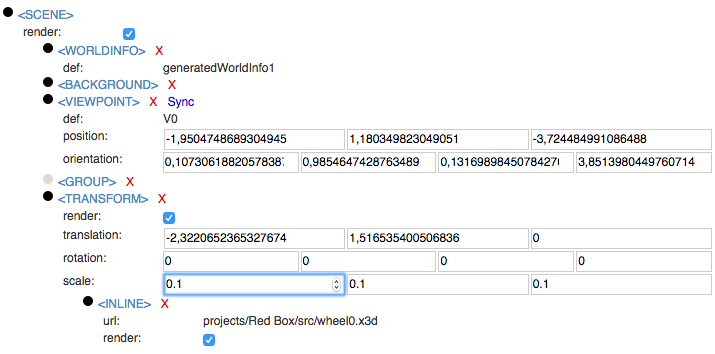
\includegraphics[width=\textwidth]{../assets/treeview.png}
  \caption{The rendered tree-view.}
  \label{fig:tree-view}
\end{figure}

\begin{figure}
  \centering
  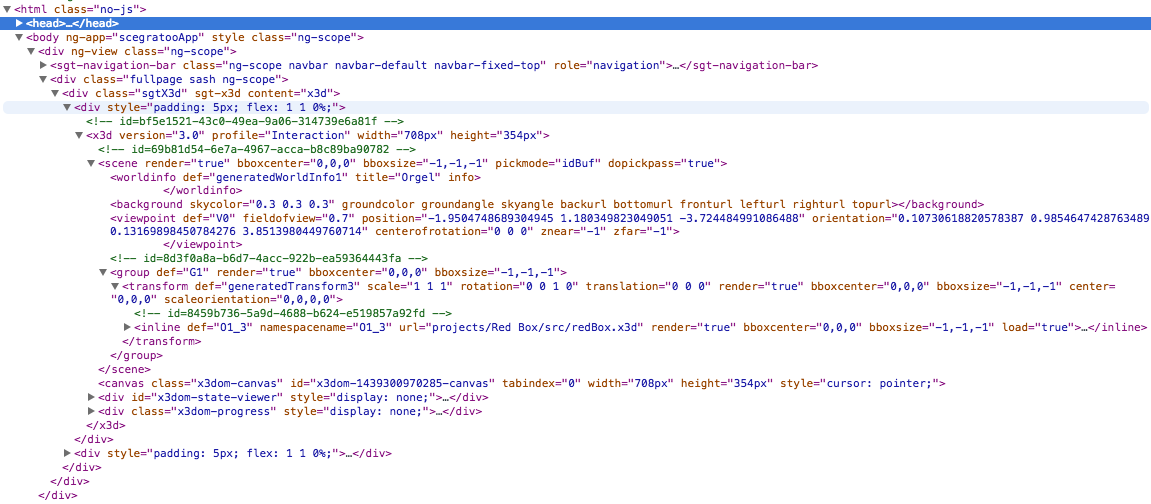
\includegraphics[width=\textwidth]{../assets/x3dom-dom.png}
  \caption{The \gls{X3D} scene inside the \gls{DOM}.}
  \label{fig:x3dom-dom}
\end{figure}

\begin{figure}
  \centering
  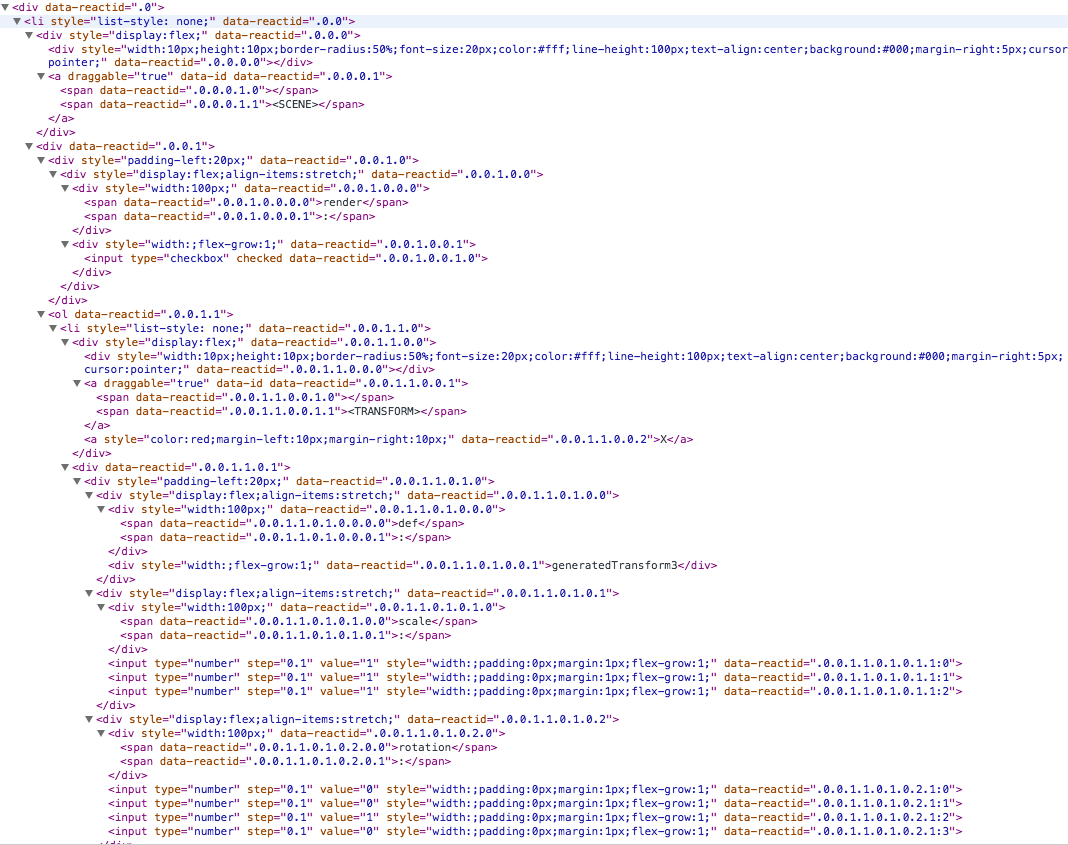
\includegraphics[width=\textwidth]{../assets/treeview-dom.png}
  \caption{About half of the \gls{DOM} elements that make up a tree-view of only three tree-view-nodes: a \texttt{scene}, a \texttt{transform} and an \texttt{inline}.}
  \label{fig:treeview-dom}
\end{figure}

\begin{figure}
  \centering
  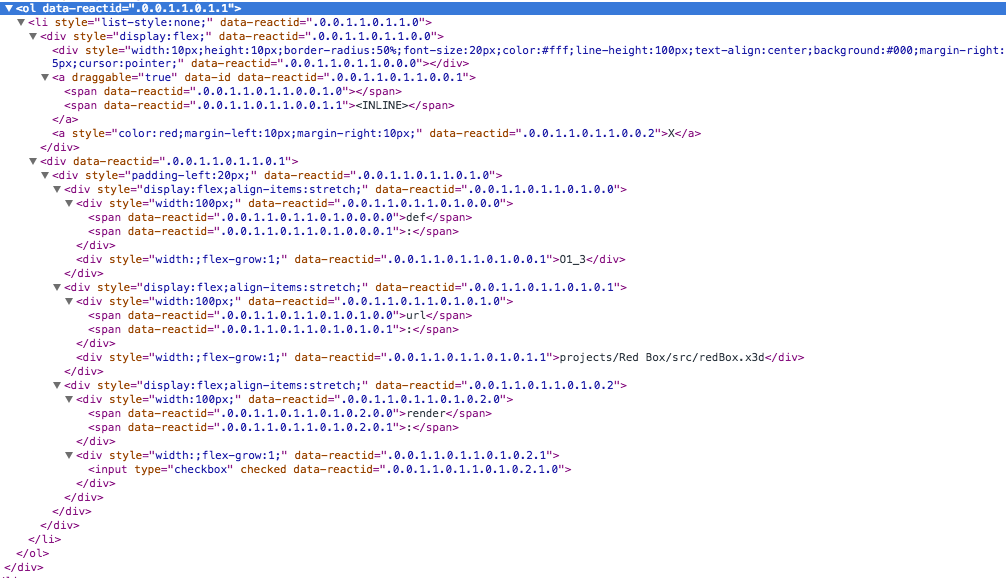
\includegraphics[width=\textwidth]{../assets/treeview-node-dom.png}
  \caption{The \gls{DOM} elements that make up a tree-view-node for an \texttt{inline}.}
  \label{fig:tree-view-node-dom}
\end{figure}

\begin{figure}
  \centering
  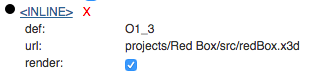
\includegraphics[width=.5\textwidth]{../assets/tree-view-node-rendered.png}
  \caption{The rendered tree-view-node of an \texttt{inline}.}
  \label{fig:tree-view-node-rendered}
\end{figure}

\begin{listing}
  \begin{minted}[breaklines,bgcolor=bg]{html}
<x3d version="3.0" profile="Interaction" width="708px" height="354px">
<!-- id=69b81d54-6e7a-4967-acca-b8c89ba90782 -->
<scene render="true" bboxcenter="0,0,0" bboxsize="-1,-1,-1" pickmode="idBuf" dopickpass="true">
<worldinfo>
</worldinfo>
<background skycolor="0.3 0.3 0.3"></background>
<viewpoint fieldofview="0.7" position="1 1 3" orientation="0.1 0.9 0.13 3.8">
</viewpoint>
<!-- id=8d3f0a8a-b6d7-4acc-922b-ea59364443fa -->
<group render="true" bboxcenter="0,0,0" bboxsize="-1,-1,-1">
  <transform render="true">
    <!-- id=8459b736-5a9d-4688-b624-e519857a92fd -->
    <inline url="projects/Red Box/src/redBox.x3d" render="true" load="true">
      <Shape render="true" isPickable="true">
        <Appearance sortType="auto" alphaClipThreshold="0.1">
          <Material diffuseColor="1 0 0" ambientIntensity="0.2" shininess="0.2"></Material>
        </Appearance>
        <Box solid="true" size="2,2,2"></Box>
      </Shape>
    </inline>
  </transform>
</group>
</scene>
</x3d>
  \end{minted}
	\caption{ \gls{X3D} example scene.}
	\label{list:x3dscene}
\end{listing}

\begin{listing}
  \begin{minted}[breaklines,bgcolor=bg]{html}
<div>
  <li>
    <div>
      <a> <span>SCENE</span> </a>
    </div>
    <div>
      <div>
        <div>
          <div>
            <span>render:</span>
          </div>
          <div>
            <input type="checkbox">
          </div>
        </div>
      </div>
      <ol>
        <li>
          <div>
            <a> <span>WORLDINFO</span> </a>
            <a>X</a>
          </div>
          <div>
            <div>
              <div>
                <div>
                  <span>def:</span>
                </div>
                <div>generatedWorldInfo1</div>
              </div>
            </div>
          </div>
...
      </ol>
    </div>
  </li>
</div>
  \end{minted}
  \caption{Example tree view structure, structure is simplified.}
  \label{list:tree-view}
\end{listing}

The aim is to keep the tree-view a consistent representation of the scene-graph.
The tree-view filters some nodes and attributes. As an example nodes contained
in an \texttt{inline} are not shown, since  SceGraToo's task is only to compose
a scene of \texttt{inlines}, not to change anything inside the \texttt{inlines}.
Also not all attributes are shown, but only the ones the user may be interested
in (such as \texttt{DEF}, \texttt{translate} or \texttt{rotate}).

One approach is to instantiate the tree-view-component with a
scene-graph-node as root node. For all child nodes the tree-view-component
instatiates new tree-view-node-components. These tree-view-node-components
create the corresponding tree-view-nodes while further traversing the
scene-graph. For each scene-graph-node a corresponding tree-view-node-component
is created. If there are no child nodes left the tree-view creation is done.
Each tree-view-node-component creates all \gls{DOM} elements necessary to represent
the corresponding scene-graph-node in the \gls{DOM}. Also each
tree-view-node-component observes its corresponding scene-graph-node for
attribute mutations and added or removed child nodes and acts accordingly.

Depending on how the scene-graph is mutated three main cases can be differentiated:

\begin{description*}
  \item[a scene-graph-node is added]
    A new tree-view-node-component is instantiated, adding all \gls{DOM} elements making up the tree-view-node to the \gls{DOM}.
  \item[a scene-graph-node is deleted]
    The corresponding tree-view-node-component is destroyed and all \gls{DOM} elements making up that tree-view-node are removed from the \gls{DOM}.
  \item[a scene-graph-node is mutated]
    The corresponding \gls{DOM} elements that make up the  tree-view-node are altered to reflect the mutation.
\end{description*}

Tree-view-nodes can also be used to edit scene-graph nodes' properties. When an
input element that contains the x value of a transformation is edited its
tree-view-node-component is notified of the change, by firing a change event to
which the component subscribed, and applies the new value to the corresponding
scene-graph-node.

It is assumed that the updates will always lead to consistent a state, where the
scene-graph and the tree node converge. It is also assumed that an application
may be buggy and in that case the synchronization process has no ability to
detect if updates lead to an inconsistent state. It also has no ability to
recover from an inconsistent state, though without the ability to detect
inconsistencies this does not really matter.

In the following the two main problems are described.

\begin{description*}
  \item[Problem 1: keeping the tree-view consistent with the scene-graph]
    The difficulty to make sure that incremental updates are error-free
    exacerbates even more when further functionality - like checkboxes for
    specific properties or saving state in the tree-view that is not part of
    the scene-graph, like the possibility to collapse parts of the tree - is
    added to the tree-view.
  \item[Problem 2: implementation effort]
    For every new feature four things have to implemented:
    \begin{enumerate*}
      \item Code for parsing the scene-graph
      \item Code to generate the tree-view-node
      \item Code to synchronize changes to a scene-graph-node to the corresponding tree-view-node
      \item Code to synchronize changes to a tree-view-node to the corresponding scene-graph-node
    \end{enumerate*}
\end{description*}

This can be greatly simplified if only the functionality for parsing the
scene-graph and creating \gls{DOM} elements to represent the parts of the scene-graph
is implemented and on every change the whole tree-view is recreated by doing
this again.

Problem 1 disappears completely, because the incremental updates are gone and
Problem 2 is reduced to the following two steps:

\begin{enumerate*}
  \item Code for parsing the scene-graph and generating the tree-view
  \item Code to synchronize changes to a tree-view-node to the corresponding scene-graph-node
\end{enumerate*}

Rerendering everything on every change is usually inefficient. Removing a big part
of the \gls{DOM} and replacing it would kick of a \emph{reflow}, which is the browser's
process of laying out the content. This process is blocking, meaning the user can't
scroll or otherwise interact with the application. \cite{reflow}

React is used to minimize the possibility of a reflow happening. React
calculates a lightweight representation of what the \gls{DOM} should be like and
compares that to what the \gls{DOM} is already. It calculates a set of patches and
only applies these to the \gls{DOM}.

From a developer's point of view the application is programmed like it is
completlely rerendered everytime something changes. But from the browser's point
of view, only a minimal set of changes, only those that are required to transform the
\gls{DOM} into the disired state, are applied, thus greatly reducing the risk of a reflow.

The code below (listings \ref{oldvirtdom}, \ref{newvirtdom} and \ref{patch}) is
for explanitary purposes to describe how react works. It does not resemble
react's implementation in any way:

\begin{listing}[H]
  \begin{minted}[breaklines,bgcolor=bg]{html}
<ol data-reactid=".0">
  <li data-reactid=".0.0">scene
    <ol data-reactid=".0.0.0">
      <li data-reactid=".0.0.0.0">transform
        <ol data-reactid=".0.0.0.0.0">
          <li data-reactid=".0.0.0.0.0.0">inline</li>
        </ol>
      </li>
    </ol>
  </li>
</ol>
  \end{minted}
  \caption{Old Virtual DOM}
  \label{oldvirtdom}
\end{listing}

\begin{listing}[H]
  \begin{minted}[breaklines,bgcolor=bg]{html}
<ol data-reactid=".0">
  <li data-reactid=".0.0">scene
    <ol data-reactid=".0.0.0">
      <li data-reactid=".0.0.0.0">transform
        <ol data-reactid=".0.0.0.0.0">
          <li data-reactid=".0.0.0.0.0.0">inline</li>
        </ol>
      </li>
      <li>group</li>
    </ol>
  </li>
</ol>
  \end{minted}
  \caption{New Virtual DOM}
  \label{newvirtdom}
\end{listing}

\begin{listing}[H]
  \begin{minted}[breaklines,bgcolor=bg]{javascript}
var li = document.createElement('li')
li.innerText = 'group'
document.querySelector('[data-reactid=".0.0.0"]')
  .appendChild(li)
  \end{minted}
  \caption{Patch}
  \label{patch}
\end{listing}

That means as long as the code that parses the scene-graph and generates the
lightweight representation of the tree-view is correct, the tree-view will
represent the current state of the scene-graph.

\paragraph{Data Binding}
\label{data-binding}

Another idea is to utilize templates and data binding. Frameworks like
angular or web components implementations like polymer
support templates and two way data binding. Following only
angular directives are examined, but the same should be possible with web
components.

An angular directive consists of a mostly logicless template and some
javascript containing logic for creating the directive or reacting to
events.

For each node a directive is instantiated which creates a template
rendering the node. Also for each child it creates a new instance of
itself.

\textbf{Example:}

The structure that is rendered is shown in listing \ref{list:templatedata}. The
\texttt{treenode} (listing \ref{list:angular1}) expands into the node name and a
\texttt{nodelist} (listing \ref{list:angular2}), that then expands into a list
of tree-nodes for each child node (listing \ref{list:angular3}), that further
expand again (listing \ref{list:angular4}). This recursive expanding stops when a
\texttt{treenode} is childless.

\begin{listing}[H]
  \begin{minted}[breaklines,bgcolor=bg]{javascript}
node: {
  name: "scene",
  children: [
    {
      name: "viewpoint"
    },
    {
      name: "worldinfo"
    }
  ]
}
  \end{minted}
  \caption{Example input data.}
  \label{list:templatedata}
\end{listing}

\begin{listing}[H]
  \begin{minted}[breaklines,bgcolor=bg]{html}
<treenode node="node">
</treenode>
  \end{minted}
  \caption{The initial template, node is the node from the data in listing \ref{list:templatedata}.}
  \label{list:angular1}
\end{listing}

\begin{listing}[H]
  \begin{minted}[breaklines,bgcolor=bg]{html}
<treenode node="node">
  <span>{{node.name}}</span>
  <nodelist ng-repeat='node in children' children='children'>
  </nodelist>
</treenode>
  \end{minted}
  \caption{The template expands itself, putting the node's name into a span and adding a nodelist directive that expands the node's children.}
  \label{list:angular2}
\end{listing}

\begin{listing}[H]
  \begin{minted}[breaklines,bgcolor=bg]{html}
<treenode node="node">
  <span>{{node.name}}</span>
  <nodelist ng-repeat='node in children' children='children'>
    <treenode node="children[0]">
    </treenode>
    <treenode node="children[1]">
    </treenode>
  </nodelist>
</treenode>
  \end{minted}
  \caption{The nodelist expands the children array and renders a treenode for every child.}
  \label{list:angular3}
\end{listing}

\begin{listing}[H]
  \begin{minted}[breaklines,bgcolor=bg]{html}
<treenode node="node">
  <span>{{node.name}}</span>
  <nodelist ng-repeat='node in children' children='children'>
    <treenode node="children[0]">
      <span>{{node.name}}</span>
    </treenode>
    <treenode node="children[1]">
      <span>{{node.name}}</span>
    </treenode>
  </nodelist>
</treenode>
  \end{minted}
  \caption{The treenode directive expands the nodes and renders their names, since there are no nodes left to render they stop.}
  \label{list:angular4}
\end{listing}


Again, this is not an accurate depiction of how angular works, it is just
for illustration purposes.

The scene-graph is traversed and for each eligible child node a new
\texttt{treenode} is created. The double braces are angular's way
to denote data-binding in templates. The data from the elements scope is
automatically inserted and kept up to date. This data binding would then
ensure that when the \texttt{treenode}'s attributes are changed the model is
kept in sync and the other way around.

\subsection{Communication}
\label{interaction}

The client comunicates with the server via a small HTTP API returning \gls{JSON}.
Making a GET request to \texttt{/projects} returns all projects stored on the server.
Making a GET request to \texttt{/projects/unicorn} returns all data about unicorn project.


% TODO: objects are missing, need to convert them to pdf
\subsection{Implementation}\label{implementation}

\subsubsection{Used Tech}\label{used-tech}

\paragraph{angular}\label{angular}

\begin{itemize*}
\item
  dependency management
\item
  resource management
\item
  less dynamic templates
\end{itemize*}

\paragraph{react}\label{react}

\begin{itemize*}
\item
  highly dynamic views (like the tree view)
\end{itemize*}

\subsubsection{Problems}\label{problems}

\paragraph{synchronization Process}\label{synchronization-process}

This design leads to brittle code that is hard to maintain and hard to
adapt to new use cases.

The first culrpit in this design is that the tree-view-controller
mutates itself.

Let's externalize the mutation observation and update capabilities into
another actor: a mutation observer.

The mutation observer can map each graph node to its corresponding tree
node and thus change the tree node to represent the matching graph node
again.

The tree-view-controller does not mutate itself anymore. All the
mutation logic that synchronizes the tree-view-controller with the
scene-graph is in the mutation observer. But the scene-graph and the
tree-view-controller can still diverge, since moving the mutation logic
from the tree-view-controller to the mutation observer does not make it
easier to reason about and thus less error prone.

Assuming that the first operation (traversing the scene-graph and
creating the tree-view-controller) is correctly implemented and
resilient, the easiest way to make sure the tree-view-controller and the
scene-graph are in sync would be to recreate the tree-view-controller
whenever the scene-graph changes.

At first sight that seems to be awfully slow, that needn't to be true.
Instead of recreating the the whole tree using {[}DOM{]} elements, a
model could be created using simple javascript objects. This virtual
tree-view-controller can then be compared to the tree-view-controller
already in the {[}DOM{]} and only the changes need to be applied.

That might sound like it's no easier than doing the synchronization
manually like in the first diagram, but the diff algorithm doesn't
actually need to know what it's diffing. Meaning it could be developed
and tested once and be used by all kinds of projects. That's one thing
react provides. The rendering pipeline looks finally like this:\\

React calls the virtual representation of what will be rendered
\emph{virtual DOM}. The other important feature of react is it's way to
build the virtual DOM. A is a factory that returns A virtual DOM node is
the return value of component's render function, the render function can
nest other virtual {[}DOM{]} nodes in its return value.

A quick examples:

\begin{minted}[breaklines,bgcolor=bg]{javascript}
  // TreeNodeAttributeList :: [Attribute] -> div
  var TreeNodeAttributeList = React.createClass({
    render: function () {
      // the scene-graph node that was passed `createElement` by the caller
      var node = this.props.node;

      var whitelist = ['def', 'diffusecolor', 'orientation', 'position', 'render', 'rotation', 'scale', 'translation', 'url'];

      var attributesToRender = node.attributes.filter(function (attribute) {
        return propsToRender.includes(attribute.name.toLowerCase());
      })

      return (
        <div>
          {
            attributesToRender.map(function (attribute) {
              return <TreeNodeAttribute attribute={a} owner={node}/>
            })
          }
        </div>
      );
    }
  });
\end{minted}

The usage of HTML tags is just syntactic sugar, it's transpiled into:

\begin{minted}[breaklines,bgcolor=bg]{javascript}
  'use strict';

  // TreeNodeAttributeList :: [Attribute] -> div
  var TreeNodeAttributeList = React.createClass({
    render: function render() {
      // the scene-graph node that was passed `createElement` by the caller
      var node = this.props.node;

      var whitelist = ['def', 'diffusecolor', 'orientation', 'position', 'render', 'rotation', 'scale', 'translation', 'url'];

      var attributesToRender = node.attributes.filter(function (attribute) {
        return propsToRender.includes(attribute.name.toLowerCase());
      });

      return React.createElement(
        'div',
        null,
        attributesToRender.map(function (attribute) {
          return React.createElement(TreeNodeAttribute, { attribute: a, owner: node });
        })
      );
    }
  });
\end{minted}

This is code is the a simplified version of the code that renders a
graph's nodes attributes into the tree-view-controller. This component
simply decides what attributes should be rendered into the tree.
\texttt{TreeNodeAttribute} is another component that will renders
different elements depending on what attribute is passed in.

Because the outputted html is only a function of its input it easy to
parse the scene-graph: 1. choose a graph node as the root 2. call the
node component with that graph node 3. if the graph node has child nodes
call the node component again with each child node and return their
return values wrapped in an element 4. if the graph node has no children
return an empty element

\subparagraph{Why the chosen approach will
work}\label{why-the-chosen-approach-will-work}

After trying different solutions it turned out the a functional solution
would also suit SceGraToo the best. First Chaplin (a backbone successor)
was used to implement SceGraToo, but soon the first version of it
suffocated under it's own complexity (probably also due to the
incompetence of its user - me). It turned out that MVC had serious flaws
when trying to use it to describe an ever changing declarative
scene-graph. The naive solution would be to observe the X3D node and
rerender the whole tree structure whenever it changed, that would also
mean to rerender every time an attribute is changed. To make that clear,
that means rerendering every time an object is moved with the mouse,
since the translation is an attribute. This thesis will not contain any
benchmarks proving that manipulating the DOM from javascript is slow,
rather than that it is left as an exercise to the reader to research it
if she wants. React solves this issue quite elegantly by creating the
dom structure in javascript and diffing it with the {[}DOM{]}, only
applying the minimum of changes to the DOM to realize the corresponding
result. That made it possible to use the X3D node of the DOM as the only
source of truth and minimize the state that needs to be kept to make the
tree-view-controller work.

A solution that handles state manually can work, but requires more
discipline and a more complicated mental model. The programmer has to
keep all side effects and cascading effects in mind when changing parts
of the program.


% !TEX root = seminararbeit.tex

\section{Conclusion}\label{results}

% Die vorliegende Arbeit beschäftigt sich mit der iterativen Entwicklung einer Augmented Reality Anwendung für das Android-Betriebssystem. Ziel dabei war es eine Anwendung zu entwerfen, die als Vorlage für die Generierung mittels der SSIML-Sprachfamilie dient. Dafür wurden ver- schiedene bereits vorhandene Frameworks auf ihre Tauglichkeit für diesen Zweck überprüft. Da- nach wurde ein High-Level Framework für Android entworfen, mit welchem es möglich ist durch minimalem Programmieraufwand eine Augmented Reality Anwendung zu erzeugen. Dieses Fra- mework dient als Adapter zu low-level Frameworks und reduziert den vom Entwickler benötigten Quellcode auf ein Minimum, wodurch eine Codegenerierung mittels domänenspezifischer Spra- chen gut umgesetzt werden kann. Leider war es nicht möglich bestimmte Eigenschaften einer Augmented Reality Anwendung umzusetzen da sie den Rahmen dieser Arbeit sprengen würde. Das Überlagern von 3D-Objekte durch ein reales Objekt, oder ein sich nach der Umgebungs- beleuchtung anpassendes Lichtsystem gehören hier zu. Außerdem wäre es möglich das Sensor System um Kollisionssensoren oder Annäherungssensoren zu erweitern. Abschließend kann fest- gestellt werden, das Hilfe des in dieser Arbeit vorgestellte Augmented Reality Framework es mög- lich ist eine performante AR-Anwendung ohne große Probleme mittels der SSIML-Sprachfamilie zu Erzeugen.
% Die vorliegende Arbeit beschäftigt sich mit der iterativen Entwicklung einer
% Augmented Reality Anwendung für das Android-Betriebssystem. Ziel dabei war es
% eine Anwendung zu entwerfen, die als Vorlage für die Generierung mittels der
% SSIML-Sprachfamilie dient. Dafür wurden ver- schiedene bereits vorhandene
% Frameworks auf ihre Tauglichkeit für diesen Zweck überprüft. Da- nach wurde
% ein High-Level Framework für Android entworfen, mit welchem es möglich ist
% durch minimalem Programmieraufwand eine Augmented Reality Anwendung zu erzeugen.
% Dieses Fra- mework dient als Adapter zu low-level Frameworks und reduziert den
% vom Entwickler benötigten Quellcode auf ein Minimum, wodurch eine
% Codegenerierung mittels domänenspezifischer Spra- chen gut umgesetzt werden
% kann. Leider war es nicht möglich bestimmte Eigenschaften einer Augmented
% Reality Anwendung umzusetzen da sie den Rahmen dieser Arbeit sprengen würde.
% Das Überlagern von 3D-Objekte durch ein reales Objekt, oder ein sich nach der
% Umgebungs- beleuchtung anpassendes Lichtsystem gehören hier zu. Außerdem wäre
% es möglich das Sensor System um Kollisionssensoren oder Annäherungssensoren zu
% erweitern. Abschließend kann fest- gestellt werden, das Hilfe des in dieser
% Arbeit vorgestellte Augmented Reality Framework es mög- lich ist eine
% performante AR-Anwendung ohne große Probleme mittels der SSIML-Sprachfamilie zu
% Erzeugen.

The presented work explores the planning and the implementation of a \gls{3D} composition tool. The created tool, \gls{SceGraToo}, enables the user to:

\begin{itemize}
  \item Upload a \gls{R3D} project,
  \item visualize it,
  \item translate, rotate and scale any object,
  \item remove objects,
  \item reorder the the objects in the the treeview,
  \item add new objects via dragging them over the tree-view and dropping them on any group or transform node,
  \item save the changed scene on the server and
  \item download it again.
\end{itemize}

And all of that is possible from within the browser.

What couldn't be implemented, due to time constraints, is a way to synchronize a scene between browser sessions and allow multiple users to change one scene.


\listoftables

\clearpage
\listoffigures

\clearpage
\listoflistings

% References (Literaturverzeichnis):
% a) Style (with abbreviations: use alpha):
\bibliographystyle{plainnat-d}
% b) The File:
\clearpage
\bibliography{seminararbeit}

\clearpage
\printindex

\clearpage
\printglossaries

\emptypage

\end{document}
